 \documentclass[pgs]{DOE}
% options = draft, pgs, endfloat, double, edit

\usepackage{setspace}
\usepackage{booktabs}
\usepackage{subfiles}

% Non-indented, bold, lightly colored text.
%
\usepackage[dvipsnames]{xcolor}
\newcommand{\highlight}[1]{{\noindent \bf \color{RawSienna} #1}}
\newcommand{\mnote}[1]{{\marginpar{\color{red} #1}}}
\newcommand{\todo}[2]{{[\color{RawSienna} #1] \color{red} #2}}
\newcommand{\myclearpage}{\clearpage}
\newcommand{\draft}[1]{{\color{TealBlue} #1}}
\newcommand{\REF}[0]{{\color{red} [REF NEEDED]}}

\graphicspath{
  {/figs}
  {../figs}
  {../../figs}
}

\usepackage{csquotes}
\usepackage{pdfpages}
\usepackage{tcolorbox}
\usepackage{ifplatform}
\usepackage{wrapfig}

\newtcolorbox{gapbox}[1]{
colframe=blue!100,
colframe=blue!100, 
colback=blue!10, 
coltitle=black,
fonttitle=\bfseries,
title={#1}
}

% The \iflinux works on Overleaf, but in MacOS I get the warning
%
% Package ifplatform Warning: 
%    shell escape is disabled, so I can only detect \ifwindows.
%
% Check the operating system and then print a message to the log file

\message{the operating system is}
\iflinux
  \message{linux (i.e., Overleaf)}
\else
  \message{not linux}
\fi

% Special commands

\newcommand{\subs}[1]{_{\mathrm{#1}}}
\newcommand{\supr}[1]{^{\mathrm{#1}}}
\newcommand{\latin}[1]{\emph{#1}}

% ===============================================
% EDIT HERE to ADD/REMOVE REMOVE COLORED COMMENTS
% ===============================================
% 
% To turn off margin notes, the extra clearpages's, and todo's
% comment in the following two commands.  To retain margin notes
% the extra clearpage's, and todo's, comment out the following three
% lines.
%
\renewcommand{\mnote}[1]{}
\renewcommand{\todo}[2]{}
\renewcommand{\myclearpage}{}

% ====== START MAIN DOCUMENT =======

\setlength{\headheight}{13.59999pt}
\addhead
  {AI-Driven Materials Discovery to Power the Space Economy}
  {Marohn, John}

\newcommand{\propname}{(PS\textsuperscript{2})\textsuperscript{2}M}

\begin{document}

% =========================
% PROJET SUMMARY / ABSTRACT
% =========================

\subfile{tex/Summary}
\setcounter{page}{1} % reset page counter


% ===================
% COVER PAGE
% ===================

\clearpage
\subfile{tex/Title}

% ===================
\clearpage
\setcounter{page}{1} % reset page counter
\section{Introduction}
\mnote{1 page}
% ===================

%
% -----------------------------------
\begin{wrapfigure}{r}{0.30\textwidth}
% \vspace{-8pt}
\centering
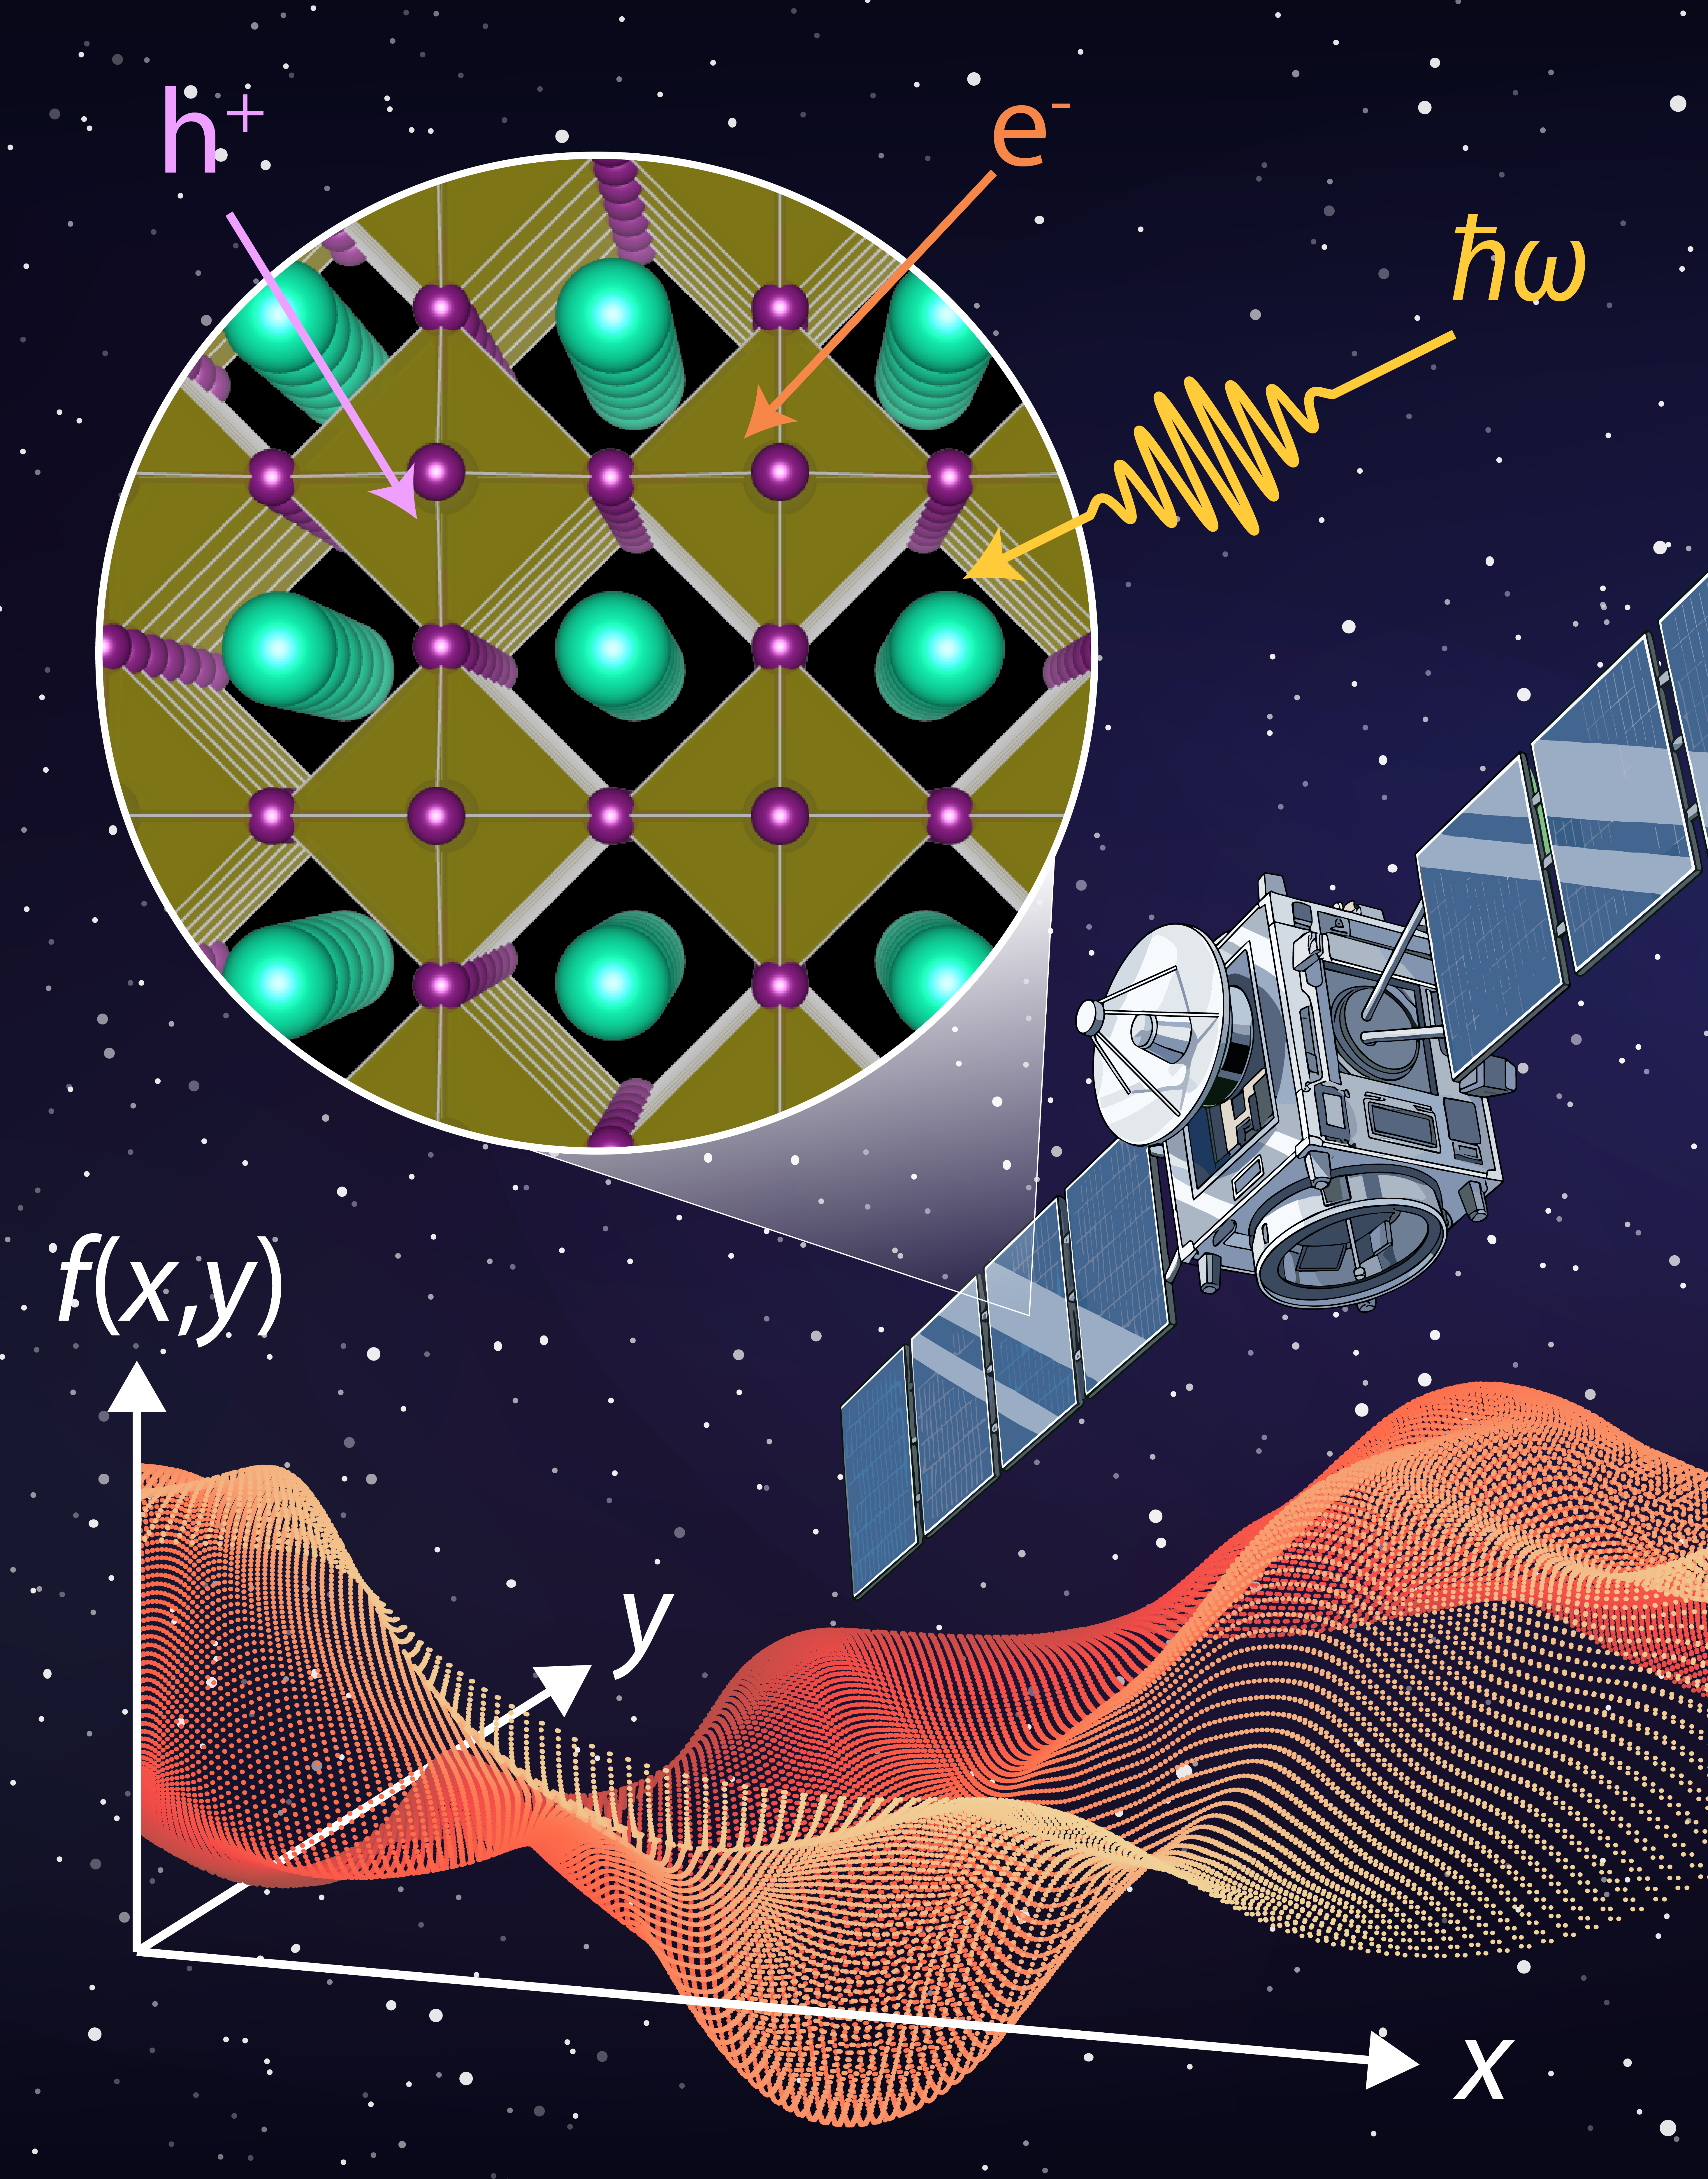
\includegraphics[width=0.30\textwidth]{Figures/Genesis_1b_hero_fig_v2.png}
\caption{\label{fig1}Project overview graphic highlighting Bayesian optimization for AI, metal halide perovskite materials, and their applications to space power.}
\end{wrapfigure}
% -----------------------------------
%
The space economy is predicted to expand significantly, and it will require equivalent amounts of on-board energy systems.
The incumbent silicon-based technology for power generation in space has a typical lifetime of only three years due to its susceptibility to damage from high-energy electrons and protons present in space \cite{Imaizumi2013may,Li2026mar}. 
Alternative technologies, like III-V absorbers, are more radiation-hard \cite{Li2021feb-space,Iwamoto2022nov}, but market supply for those materials is sold out for the next three years \cite{Powers-Riggs2025jul}.
This limited supply chain, and difficulty with scaling to large volume, drives up the price and accessibility of III-V materials.
Launch costs make it difficult and expensive to develop new materials robust enough to survive the extreme environment of space.
\textit{The advent of AI and Machine Learning (ML) for materials discovery and processing has the potential to dramatically reduce development time for new semiconductors for space-power generation.}
%
% -----------------------------------
% \begin{wrapfigure}{l}{0.25\textwidth}
% \vspace{-8pt}
% \centering
% %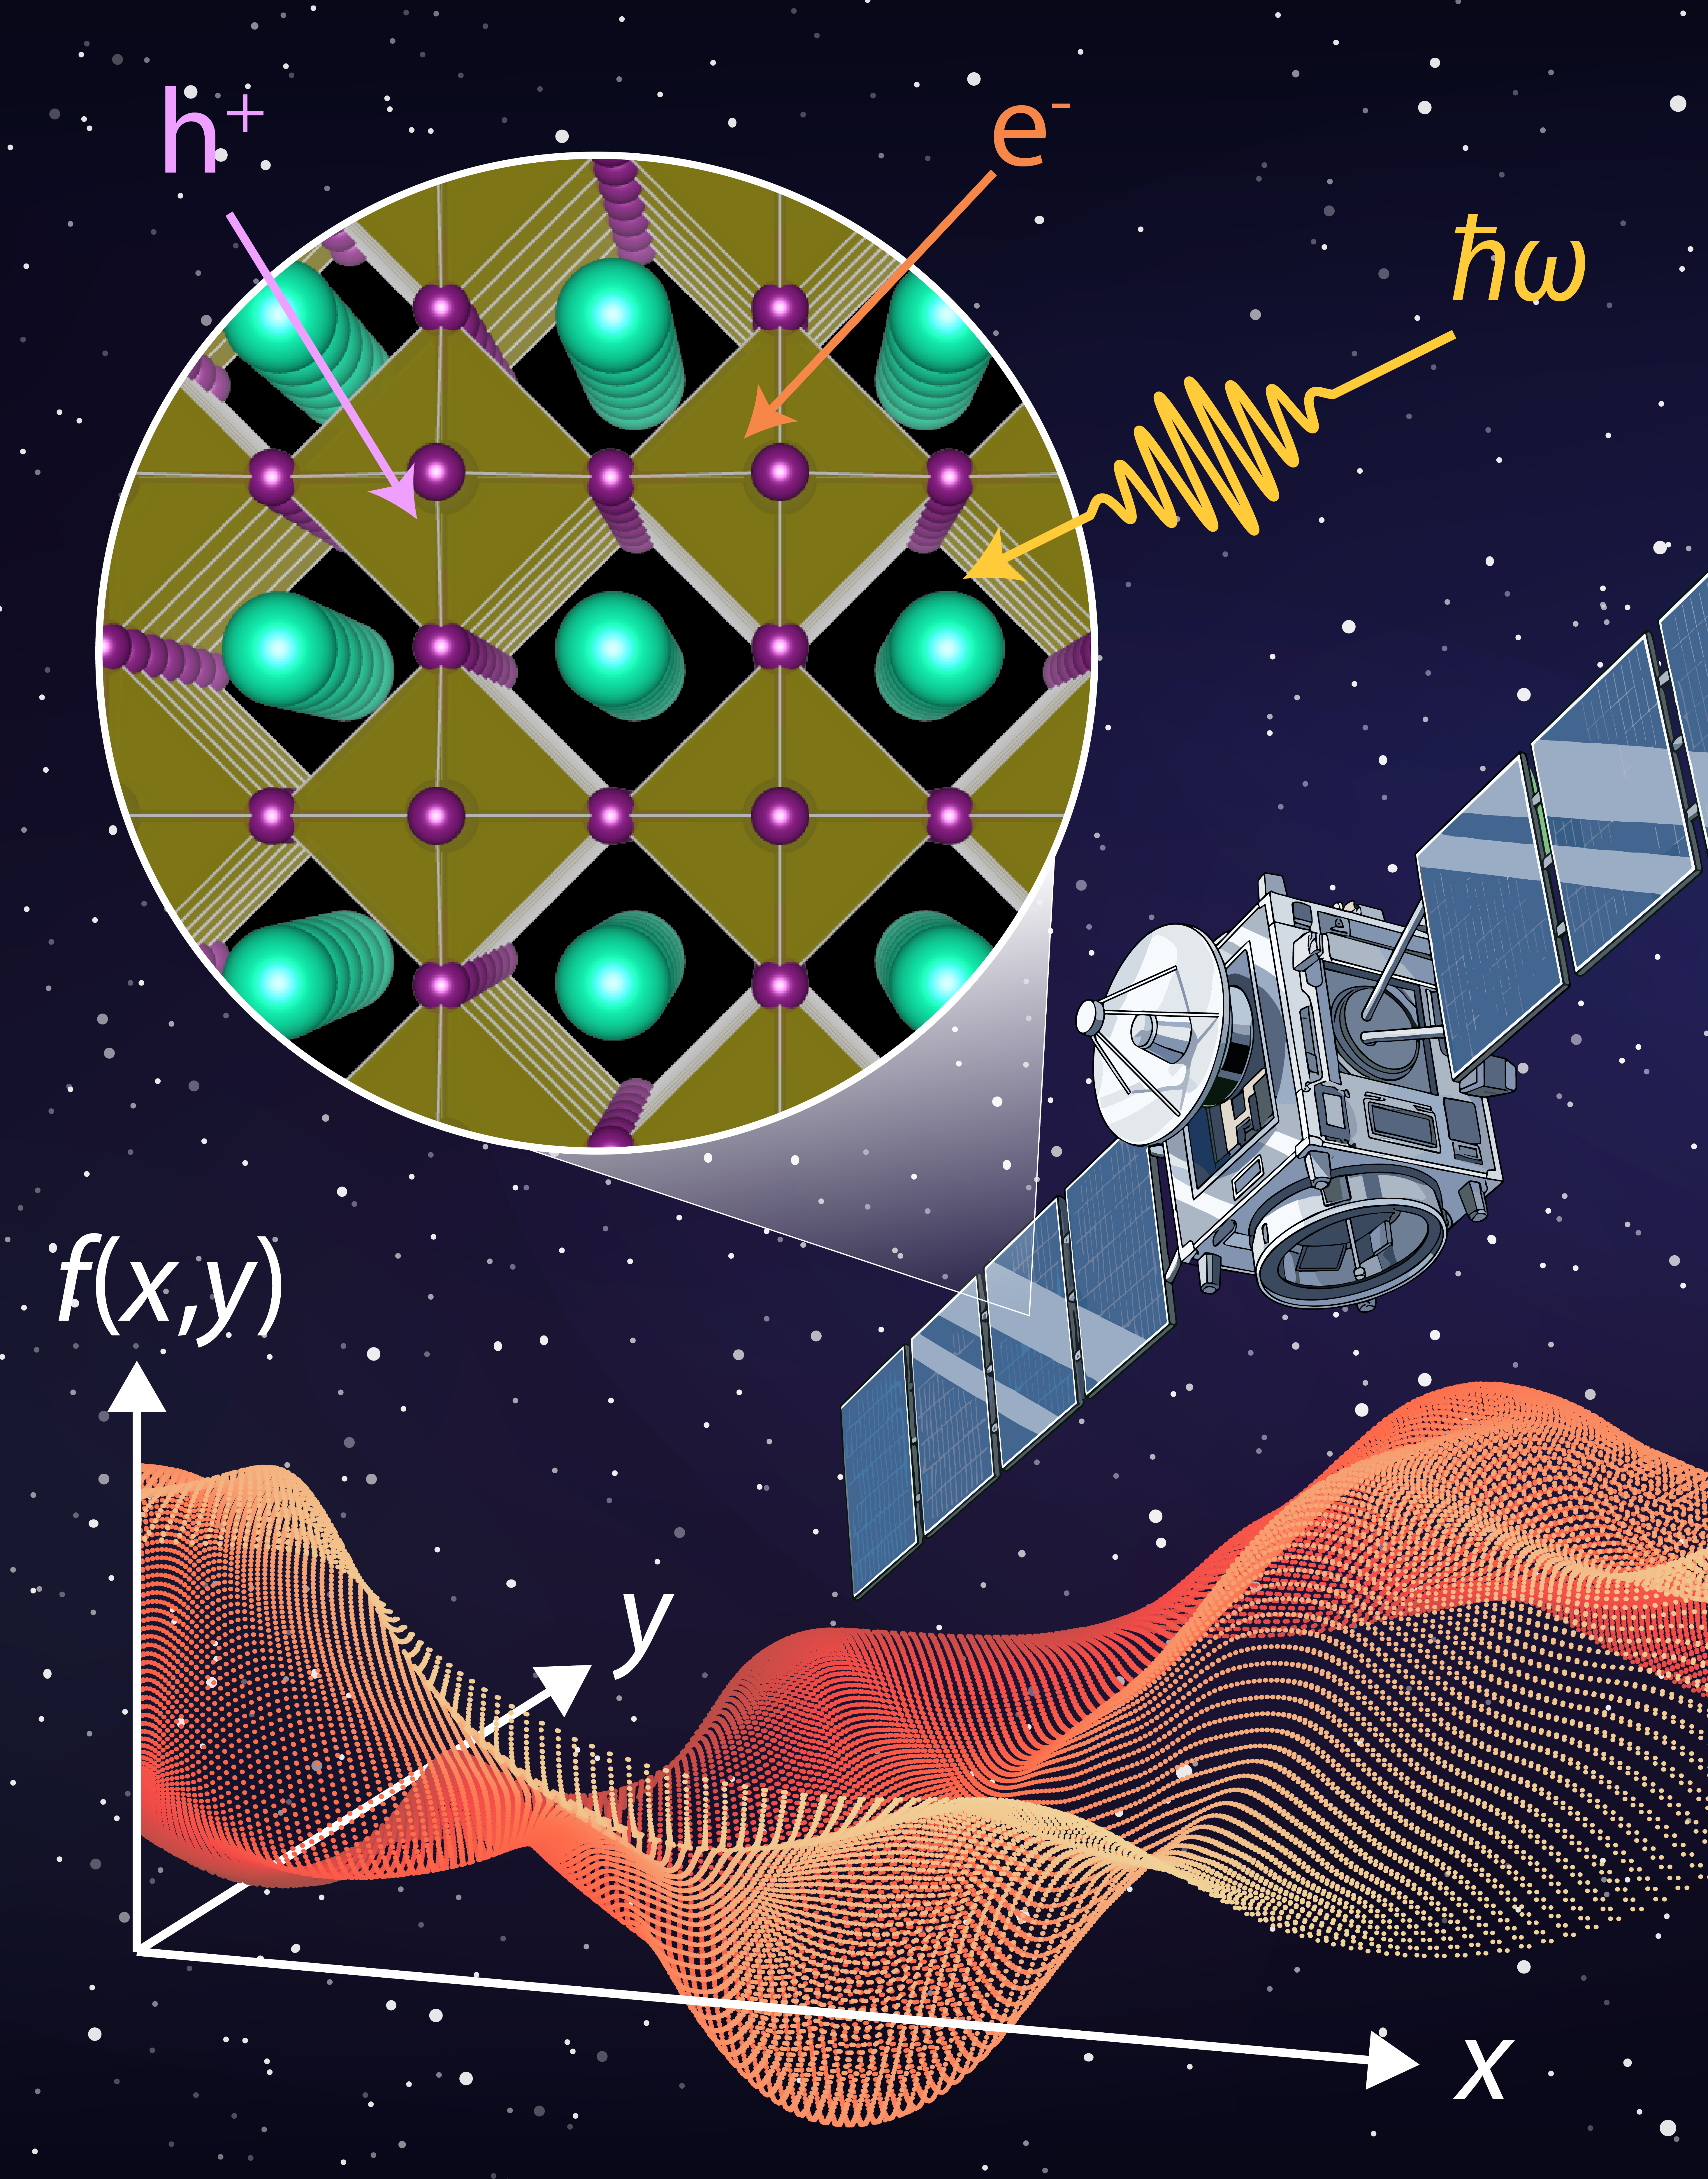
\includegraphics[width=0.35\textwidth]{Figures/Genesis_1b_hero_fig_v2.pdf}
% 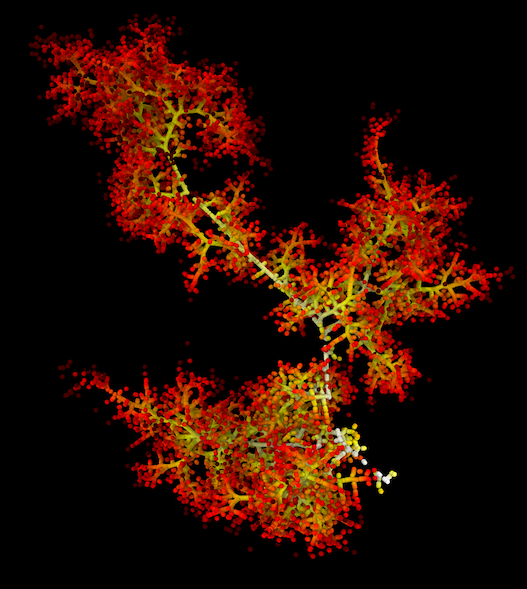
\includegraphics[width=0.25\textwidth]{Figures/tungsten_cascade_200keV.png}
% %\caption{\label{fig1}Project overview graphic highlighting Bayesian optimization for AI, metal halide perovskite materials, and their applications to space power.}
% \caption{\label{fig1}Forging radiation-resilience with AI: 
% Radiation damage in tungsten from the 240~GB CascadesDB MD simulations. Dots:individual atoms; colors: kinetic energy. The image is about 30~nm wide.}
% \end{wrapfigure}
% % -----------------------------------
% %

Metal halide perovskite (MHP) semiconductor materials have shown significant promise for space power in the form of panels or nuclear batteries for compact high-energy-density applications \cite{Song2026feb}.
% MHPs have highly tunable bandgaps by varying their \ce{ABX3} composition. %
%, and there exist numerous methods to control grain size, termination, and phase stability. 
MHPs exhibit unique resilience to radiation damage due to their mechanically ``soft'' crystal lattice \cite{rosales_leveraging_2023,Yin2014feb,Walsh2015feb,Lang2016oct,Kang2017jan,Brandt2017jun,Cahen2021nov,Miskin2025jun, ericksonFullDeviceEvaluation2025}.
This structural softness dissipates energy from energetic particle impacts through dynamic fluctuations and precessional dynamics of the octahedral network, facilitating rapid, intrinsic self-healing \cite{kirmaniUnravelingRadiationDamage2024, miskinHowSoftMetal}.
MHP materials can withstand a proton dosage three orders of magnitude higher than silicon \cite{Lang2016oct,Miyazawa2015jun}. 
They are uniquely amenable to fabrication in space, using vacuum processing \cite{Liu2013sep,Wang2018oct}, which is difficult to imagine for incumbent technologies.
Most studies on MHP materials for space are centered on materials that have been developed to survive the stressors of terrestrial applications. 
Despite their promise, there are limited studies on how perovskite chemistry and processing affects radiation hardness, a critical attribute for space power.



% Highlight other AI/ML in addition to PAL 2.0
% PAL 2.0 "developed but unproven"
% DOE Genesis mission motivated by AI LLM
% Pitch Lawler's SciLM

\textit{The goals of this proposal are to use AI to create a new class of radiation-hard metal halide perovskite semiconductors and to quantify the advantage offered by AI in meeting this materials-development challenge.}
Our team is uniquely positioned to achieve this goal. This proposal builds on \highlight{Clancy}'s powerful and interpretable Bayesian-optimization framework (PAL) \cite{Priyadarshini2024,Raguraman2024jun,Raguraman2025oct} for materials composition and process discovery and state-of-the-art machine-learned interatomic potentials (MILP) \cite{cao2025migrationprobegeneralizablebenchmark}
in molecular dynamics (MD) computations to study radiation damage dynamics.
%The framework incorporates inputs from both ab initio calculations and experimental measurements, can jointly optimize for multiple target material properties with uncertainty quantification, and works well with small datasets.
\highlight{Lawler} will develop a transformer-based structured scientific language model, similar to MatMCL \cite{wu2025versatile}, filling gaps between pre-training datasets through modeling.
This model connects our rich experimental and MD data to PAL. 
The NLR team will produce MHP materials and represent the deepest knowledge in halide perovskite synthesis, durability, and characterization in extreme environments in the world (\highlight{Wheeler} and \highlight{Witteck})\cite{noauthor_nlr_2026,witteck_reducing_2024, prince_sustainability_2025,doi:10.1021/jacs.8b04984}.
\highlight{Marohn} has developed unique, high-throughput, non-contact electrical scanning probe methods to quantify electronic and ionic charge density and conductivity of as-fabricated films in the dark and under illumination \cite{Tirmzi2017jan,Dwyer2017jun,Tirmzi2019jan,Tirmzi2020jun,Dwyer2019jun}. 
% \draft{PAL  will learn from multimodal datasets (property measurement scalars, x-ray diffraction spectra, time-resolved photoluminescence time series and MD crystal graphs) to predict improved processing conditions with uncertainty quantification. We will synthesize a perovskite device at least as radiation-hard as any III-V semiconductor within 6 months, far faster than current approaches to synthesizing such devices. \todo{Marohn}{Ref. for current rate of radiation-hard device design speeds}.I don't think this draft section is needed. It is all covered in the following section. - LW}

%Deringer2019,Chen2023nov, Chen2024apr

% ==========================
\section{Project Objectives}
\mnote{0.5 pages}
% 
% Project Objectives (approximately 0.5 page): Provide a clear and concise statement of
% the specific objectives of the proposed project. Address how the objectives align with the
% chosen focus topic and lead to an AI advantage.
%
% ==========================
The proposed work represents a high-profile test case for AI/ML to dramatically reduce the amount of experimental work to process new materials for space. 
Our Phase I objective is to use predictive AI/ML algorithms to reveal optimal compositions and processing conditions that yield radiation-hard MHPs. 

% ----------------
\begin{tcolorbox}[
    width=4.25in,
    center,
    colframe=gray,
    colback=gray!10,
    coltext=black]
    
    By month 6, we will predict and process semiconductors with radiation hardness greater than that of III-V semiconductors.
\end{tcolorbox}
% ----------------

MHP manufacturing involves a large parameter space: 
(1) \emph{stoichiometry} (2 variables): for Cs$_x$FA$_{1-x}$Pb(I$_{y}$Br$_{1-y}$)$_3$, at 1\% stoichometric resolution, we have $10^4$ independent choices for $x$ and $y$; 
(2) \emph{processing} (5 variables): choice of solvents, solvent ratio, precursor concentration, spin rate, and spin duration; 
(3) \emph{crystallization} (3 to 5 variables): either an \ce{N2} gas quench (pressure, start time, and duration) or an anti-solvent quench (solvent identity, volume, dispense time, and rate). 
% jam99: I count the dimensionality of the parameter space as 
%  N = 2 (stoich) + 5 (processing) + 3 to 5 (cryst) = 10 to 12
To optimize parameters, we could perform a 2-level search; common practice would be to perform a Plackett-Burman search \cite{Plackett1946jun} (20 experiments) to identify the important variables, then resolve interactions among the survivors with either a Fractional Factorial search \cite{Box1961aug} (16 to 64 additional experiments at Resolution V for 5 to 7 surviving factors) or a Derivative Free Optimization \cite{Oh2025dec}.
However, 2-level searches assume a linear dependence on the parameters, which we expect is a poor assumption for most of the variables in the MHP manufacturing parameter space (\emph{i.e.}, stoichiometry, solvent identity, solvent ratio, and \ce{N2} gas quench start time).
At the other extreme, a 10-level Full Factorial Design of Experiment search \cite{Lamberti2022mar} of this 10- to 12-dimensional space requires $\geq 10^{10}$ experiments.
The optimal parameter search strategy for optimizing radiation hardness is presently unknown, but it probably lies closer to the Full Factorial limit. 

% ----------------
\begin{tcolorbox}[
    width=5.50in,
    center,
    colframe=gray,
    colback=gray!10,
    coltext=black]
    
    We hypothesize that including multi-modal measurements of material properties in the surrogate model will reduce exponentially the number of terrestrial radiation hardness experiments required to optimize the metal halide perovskite material.
\end{tcolorbox}
% ----------------

 AI/ML inputs will include target stoichiometry, processing parameters, and experimental measurements of properties, e.g., film morphology, atomic lattice spacing, actual stoichiometry, and steady-state and transient electronic and ionic conductivity. The same trained model applies when the deposition method changes. Initial training uses spin-coating and evaporation. Spin-coating recipes rarely transfer one-to-one to scalable slot-die or spray coating \cite{Hamukwaya2022feb,Jafarzadeh2026apr}, but AI bridges this gap by evaluating a few new measurement points and adjusts parameters for the new process.

% Lance Wheeler:
% 
% \mnote{\draft{How many experiments does the "common practice" require? Did I count 20 + 64*7 = 468?} \draft{It would great to put a number on this. How many fewer experiments than the "common practice?" This is the why AI part that I think we need to nail down quantitatively} }


% The MHP chemical space and processing space contains $\geq 10^7$ combinations and is simply too large to sample by trial and error. 
% In this case, Design of Experiment (DoE) optimization is usually applied.
% For seven variables, DoE would require at least $2^2 = 128$
%  We assert that our approach has two advantages over DoE optimization.
% 
% We will achieve AI advantage by (1) identifying which materials properties best predict radiation hardness, and should therefore be used for in-line optimization, (2) identifying which stoichometries and processing conditions yield materials with the best radiation hardness. (3) The Bayesian model significantly reduces the number of samples needed compared to the DoE. \todo{Paulette}{ add metric here} (4) The trained AI model applies directly to a different processing environment to make process transferability easier. Our AI model trains initially on spin-coating and evaporation processes. A spin-coating process rarely transfers directly to a scalable slot-die or spray coating process. The AI accounts for this discrepancy by evaluating a few new measurement points and adjusting the parameters for the scalable slot-die or spray coating process.

% 
% We define AI advantage as the size of the profitable chemical and processing space determined by AI/ML relative to a blind search. 
% If, for example, AI/ML after one iteration has reduced the space to $10^{3}$ likely profitable stoichometry and processing combinations, then the AI advantage would be $10^7 / 10^3 = 10^4$.
% The proposed work directly resolves a persistent deficiency in existing AI/ML approaches to materials optimization --- their inability to provide physical insight.
% The proposed work will represent a high-profile test case of a new, quantitative, and transformative paradigm in AI-driven materials manufacturing.


% ===============================
\section{Data Sources and Models}
\mnote{0.5 page}
%
% Data Sources and Models (approximately 0.5 page): Describe which existing or new
% data sources will be used. Address your team’s access to the data. If applicable, indicate
% which AI models or frameworks will be used in your proposed project. Do not include a
% description of computing resources and the means by which you will secure an allocation
% timed to your performance period; this should be done in Appendix 2.
% 
% NOTES: 
% - Electron testing at Neobeam ($10k per run)
% - Most testing using electron beam testing is empirical for GaAs, 
%   which does not do a good job capturing radiation hardness of perovskites. 
% 
% ===============================

\subfile{tex/Section-V-table}

We will leverage non-contact measurements of MHP materials generated specifically for this project to ensure high data quality; see Table~\ref{table:sources}. 
Samples with varied stoichiometry (Cs, FA; I, Br) will be prepared under diverse processing conditions (\textit{i.e.},\ solvent, spin conditions, \ce{N2} flow rate, quench timing, and quench duration). After synthesis, we will perform a baseline assessment of material properties.
The resulting MHP films will be subjected to proton and electron irradiation (\SI{e15}{\per\square\centi\meter}) and their properties will be reassessed. 
We will perform 30 measurements/week of structure and morphology (SEM, XRD), stoichiometry (EDX), and optical properties (UV-Vis-NIR absorption, SPRL, tr-PL) and 15 measurements/week of steady-state and transient electronic and ionic conductivity (MC, TRMC, BLDS, pk-EFM, and nc-FvT). Our ability to quantify the density and conductivity of both electronic and ionic carriers in a non-contact measurement of as-fabricated films is unique.
Scalar data can be input into the Bayesian PAL 2.0 framework directly, whereas vector data will be coupled in through a machine-learning transformer model, which reduces data dimensionality. 
%Michel: looks good! \todo{Michael}{John: Is the last sentence an ok summary of what you plan to do?  The discussion of scalar and vector data could go below.}
We will pre-train the transformer model on overlapping datasets that link different types to each other using modeling to fill in any gaps, such as the XRD calculations on CascadesDB crystal structures presented in Fig.~\ref{fig2}. Sources of such pre-training data include the \href{https://github.com/blaiszik/awesome-matchem-datasets}{Awesome Materials \& Chemistry Datasets}, CascadesDB, and ionic conductivity electrolyte data from Ref.~\citenum{zohair2025chemical}.
As needed, we can train on outputs from other models, \textit{e.g.}, MACE \cite{wu2025versatile,wu2023molformer,wang2024graphformer,choudhary2024atomgpt}.

% =====================================
\section{Proposed Research and Methods}
\mnote{1.5 page}
%
% Proposed Research and Methods (approximately 1.5 pages): Provide a clear research plan for a nine-month project and describe the proposed activities and methods. Include enough technical details to evaluate the impact of the proposed activity. For each activity, indicate the responsibility of the key investigator(s) and the associated budget.
% If the proposed application is building on an existing, currently funded DOE project,
% describe how the submitted application leverages that work and is distinct from existing funding.
% =====================================

Our approach combines AI/ML with MHP processing and characterization into an iterative workflow.
See Fig.~\ref{fig3}.

%
\begin{enumerate}
    \item Prepare MHP thin-film samples using automated spin-coating and vacuum deposition under a variety of carefully controlled processing and synthesis conditions.
    \item Perform multi-modal characterization of material properties; see Table~\ref{table:sources}.
    \item Use the AI/ML methods detailed below to predict properties from synthesis and processing conditions.
    \item Expose the materials to high-energy electrons and protons to mimic radiation exposure in Earth orbit.
    \item Perform multi-modal characterization of material properties after exposure, using steady-state and transient electronic and ionic conductivity as a proxy for radiation hardness.
    \item Use AI/ML to develop a surrogate model, with multi-modal materials properties as inputs, and use this model to select stoichometries and processing conditions yielding MHPs with high radiation hardness.
    \item Repeat the radiation-hardness optimization cycle, Steps 1 to 6, iteratively twice in nine months.
\end{enumerate}

% ----------
\begin{figure}
\centering

\includegraphics[width=0.95\textwidth]{Figures/perovskite_space_v3.pdf}
\caption{\label{fig3}The multimodal closed-loop active learning cycle accelerates the discovery of radiation-hard perovskites. 
An AI framework utilizing XGBoost and PAL 2.0 predicts optimal material parameters \cite{Priyadarshini2024} from scalar data. 
Automated robotic spin-coating synthesizes a diverse sample library by systematically varying composition and morphology.
Multi-modal characterization, including XRD, SRPL, TRPL, and BLDS is followed by high-energy electron (1 to 5~MeV) and proton (1 to 2~MeV) radiation testing following AIAA S-111A protocols \cite{AIAA2014}. 
Post-irradiation characterization quantifies defect formation and intrinsic structural recovery.
A multi-modal transformer then feeds this empirical data back into the surrogate model to continuously refine subsequent material predictions.}
\end{figure}
% ----------


\subsection{AI/ML approaches}.
\textit{Bayesian optimization} is highly effective, even with small datasets. It incorporates physico-chemical information through both \textit{ab initio} and experimental data, and offers uncertainty quantification. \cite{Herbol2018sep}
We developed a highly interpretable Bayesian code base, the Physical Analytics Pipeline 2.0 (PAL 2.0), \cite{Priyadarshini2024} which reveals correlations of specific properties with a user-chosen objective.
We have used PAL 2.0 successfully to study metal halide perovskites, polymers, metal alloys, and metal organic frameworks, \textit{etc.}
% For example, we recently designed an orthopedic-screw alloy with record-high strength and acceptably low corrosion in only three rounds of optimization. \cite{Raguraman2025oct}
% Our proposed studies will be conducted as either a single or multiple  optimization or in a ``closed loop'' mode.
% The approach can be used either with experimental data as input or with ``synthetic'' computational data. 
Here, PAL 2.0 will enable us to sift through potential stoichiometries, processing conditions, and material properties to achieve our radiation hardness objective. 
In each iteration, PAL 2.0 makes predictions of improved materials based on its existing training data; 
it then makes updated predictions of materials with even better radiation hardness,
and the iterative cycle will continue. 
% We will fold vector and image data into PAL 2.0 using the transformer model to learn the relationships between the inputs to PAL and these other data types through pretraining and fine-tuning on datasets with overlapping data modalities.

%these materials will be fabricated, tested, and the test results added to the data base.

% ---------------
%
\begin{figure}
\begin{minipage}{0.64\textwidth}
    \centering
    \vspace{-0.5cm}
    
\includegraphics[width=\textwidth]{Figures/fig2.pdf}
\end{minipage}
\hfill
\begin{minipage}{0.35\textwidth}
    \caption{\label{fig2} Preliminary results: predicting damaged sample XRD from calculated XRD of crystals in the CascadesDB dataset and learning conductivity--temperature plots of SMILES encoded formulations in Li-ion electrolytes.  
    {\bf a.} Architecture: a multilayer perceptron (MLP) fed to a 1-D convolutional neural network. 
    {\bf b.} Mean square error (MSE) loss for training and validation sets. 
    {\bf c.} The trained model predicts XRDs from categorical inputs (material composition, lattice type) and continuous inputs (lattice parameter, temperature, PKA energy, sample volume). 
    {\bf d.} and {\bf e.} A transformer model's prediction of conductivity temperature curves by tokenizing the SMILES-temperature-conductivity dataset in Ref.~ \citenum{zohair2025chemical}. 
    M.\ Lawler (unpublished).}
\end{minipage}
\vspace{-20pt} % Manual adjustment
\end{figure}
%

\textit{Scientific Language model architecture}. 
By tokenizing data from composition, processing parameters, XRD, photoluminescence, ionic conductivity, etc., and forming into (string, value) tuples, we will complement PAL 2.0 by training a transformer model capable of learning relationships between diverse data modalities (\textit{e.g.}, composition, processing parameters, XRD, photoluminescence, ionic conductivity, \textit{etc.}) and forming them into (string, value) tuples. 
For example, the transformer model in Fig.~\ref{fig2}, produced as preliminary data for this proposal, was trained on an Li-ion electrolyte dataset with SMILES--percentage pairs describing a formulation, together with temperature and conductivity. Atoms/ions in SMILES strings were each given a token as well as the branching parentheses.
Strings for temperature and conductivity were captured by one token each. 
Other than tokenization, the model will use standard next-token prediction encoder-only (BERT) \cite{Devlin2019may} or decoder-only (GPT) transformer architecture.


\textit{Development of MLIPs for dynamic properties}.
Non-equilibrium dynamic properties are critically important for radiation hardness, but are poorly predicted; errors in calculated migration energies, for example, can exceed 10~eV \cite{cao2025what}.
Instead, we will use Dual-Level Explainability (DUAL-X), our MLIP framework that interprets machine-learned force fields at both the model level (attribution-based feature importance) and physics level (mapping learned representations back to chemically meaningful descriptors) \cite{cao2025what}.
Our Migration-Probe Benchmark will use atomic migration pathways as a diagnostic probe to reveal when specialist versus generalist MLIPs fail on non-equilibrium configurations, exposing transferability failures that standard equilibrium benchmarks often miss. 

% Applied to Cr-doped Sb$_2$Te$_3$ systems, this approach was featured at the AAAI 2026 XAI4Science Workshop as a Spotlight (top 3\%).  
% as presented at NeurIPS 2025 AI4Mat Workshop (Spotlight).

% We critically evaluated the efficacy of machine-learned interatomic potentials (MLIPs) to capture dynamic properties of doped 2D materials. We found the well-received MACE-based foundation models perform unexpectedly well in predicting equilibrium properties, especially if fine-tuned over a range of temperatures. However

%\draft{We will complement PAL 2.0 with a transformer-based ``Scientific Language Model'' (SciLM), a foundation model that fuses multi-modal characterization (XRD, SRPL, TRPL, BLDS, ionic conductivity) into learned features supplied to PAL---directly addressing Genesis Topic 1-B's call to integrate multi-modal datasets---and is pretrained on the existing perovskite literature to provide PAL a learned chemistry prior absent from hand-crafted features alone. SciLM also functions as a generative proposer of structurally novel candidates---new additives, cation/anion combinations---outside PAL's current discrete parameterization, providing a learned source of search-space expansions.}



% \begin{wrapfigure}{l}{0.4\textwidth}
% \centering
% 
\includegraphics[width=0.4\textwidth]{Figures/Inverse_solution_fig.pdf}
% \end{wrapfigure}
%
% ---------------

\subsection{MHP processing and characterization}.
We will prepare samples by both automated spin-coating and vacuum deposition.  
% Spin-coating is suitable for quickly creating \si{\centi\meter\squared} proof-of-concept devices on metal-coated glass substrates with varying stoichiometry, whereas vacuum deposition is a higher fidelity but slower process that can be scaled to \si{\meter\squared} devices and applied directly in space.
% Spin-coating suffers from lack of reproducibility, but this has been tamed at NLR by employing distinct dry boxes for ink preparation and robot-automated spin-coating and using gas quenching instead of solvent quenching in the spin-coating step. Automated Spin-coating will quickly generate samples for radiation-hardness testing and AI/ML training and optimization.
The NLR team will first synthesize an array of MHP samples across a diverse compositional library using automated robotic spin-coating. 
The generated films explore specific mixed-cation and mixed-halide systems, such as Cs$_{x}$FA$_{1-x}$Pb(I$_{y}$Br$_{1-y}$)$_3$.
The robotic platform systematically varies the A-site cation (Cs, FA) and X-site halide (I, Br) ratios alongside specific passivation additives to control grain boundary termination. 
The AI models dictate this initial sampling using a Design of Experiments approach, paving the way for the active learning loops.
In parallel, the NLR team will prepare samples via vacuum evaporation; NLR has developed a robust vacuum evaporation process with control parameters including temperature, pressure, and gas flux that are highly reproducible and automatically logged, providing an even higher fidelity parameter space for AI/ML training and optimization.

\subsection{Property characterization}.
The NLR team will characterize samples using optical microscopy, 
XRD, SRPL, tr-PL, and steady-state and TRMC. 
Cornell will evaluate samples using energy-dispersive XRD and SEM and use electrical scanning probe methods to quantify electronic and ionic conductivity in the dark and under illumination.
Broadband local dielectric spectra  \cite{Labardi2016may,Tirmzi2019jan,Tirmzi2020jun,Dwyer2019jun}(BLDS) will be analyzed with a microscopic model \cite{Lekkala2012sep,Lekkala2013nov} to obtain electronic and ionic charge density and conductivity (hence mobility).
Fitting friction versus time (nc-FvT) \cite{Tirmzi2017jan} and pk-EFM data \cite{Dwyer2017jun} will yield the lifetime of photo-induced ionic and electronic carriers, respectively.

\subsection{Radiation testing and follow-up characterization}.  
NLR will conduct rigorous irradiation testing on the samples, 
exposing the materials to high-energy electrons and protons that replicate space environments. In-house NLR facilities handle proton-testing to enable in-depth analysis of radiation effects on the MHPs, and electron testing will be performed externally at NEO Beam Alliance Inc. The testing methodology incorporates established AIAA S-111A protocols \cite{AIAA2014, hanAdvancingPerovskiteSolar2025} and utilizes guided energy-tuned dual irradiation techniques. \cite{kirmaniUnravelingRadiationDamage2024, kirmaniCountdownPerovskiteSpace2022}
Cornell will evaluate the materials over several days following irradiation to quantify long-term defect-healing and changes in ionic conductivity.

\subsection{AI/ML feedback loop}.  
This information-rich, multi-modal data, supplemented with MD simulations, will be fed to PAL. 
The data encompass synthesis parameters, baseline properties, radiation-induced defect formation, and subsequent healing rates. PAL then navigates the vast MHP compositional space, typically optimizing using less than 15\% of the search space.
This optimization allows us to predict the most radiation-hard perovskite chemistries and processing conditions from a ranked list of candidate compositions and processing variables, testable in the next ``closed loop'' iteration.


\section{Milestones}
\mnote{1 page}
%
% Milestones in the Nine Months (approximately one page): Provide a list of clearly
% defined and measurable milestones of the project.
% 
% =====================================


% Aggressive timetable!


% VERSION 1 (Lance and Robert)
% ============================
%
% 
% \begin{table}[h]
% \centering
% \caption{Phase I Project Milestones}
% \renewcommand{\arraystretch}{1.3}
% \begin{tabular}{p{0.15\linewidth}p{0.8\linewidth}}
% \hline
% \textbf{Timeline} & \textbf{Technical Milestone} \\
% \hline
% \textbf{Month 1--3} & NLR synthesizes the initial library of 160 baseline MHP films using robotic spin-coating. Cornell completes pre-irradiation XRD, TRPL, and BLDS characterizations. \\
% & AI Team does.. \\
% \hline
% \textbf{Month 4--6} & Complete the first round of electron and proton irradiations. The team feeds the post-irradiation characterization data into the PAL 2.0 Bayesian optimization framework. AI Team executes the first active learning loop to predict the next generation of optimal $ABX_{3}$ chemistry and process conditions. \\
% \hline
% \textbf{Month 7--9} & NLR synthesizes AI-predicted high-hardness MHP candidates. Complete final cycle of radiation testing. Add new data into the database and retrain the AI surrogate model. Make new AI predictions and the cycle restarts. \\
% \hline
% \end{tabular}
% \end{table}

% VERSION 2 (John)
% ================
% 
% 6 months is 26 weeks
% 9 months is 40 weeks
%
% Cornell has throughput of
% - 30 samples/wk or 120 samples/month SEM, EDX, XRD
% - 15 samples/wk or 60 samples/month for EFM

% BY MONTH?

% Below we show the expected weekly cadence for the \emph{first round} of sample growth and characterization.
% We identify work to be completed each week at the National Laboratory of the Rockies (NLR), Cornell University (CU), and the Johns Hopkins University (JHU). Measurement acronyms are defined in Table~\ref{table:sources}.
% In week 4, NLR will initiate sample growth using vapor deposition; characterization of these samples will proceed in parallel with the analysis of the spin-cast samples.

% % ------------
% \vspace{-8pt}
% \begin{center}
% \begin{tabular}{rrl}
% \toprule
% wk & group & milestone completed \\
% \midrule
% 2 & NLR & 60 metal-halide perovskite films synthesized using robotic spin coating \\
% 4 & NLR & Pre-irradiation morphology, optical spectroscopy, and electronic conductivity \\
%  & & \quad (optical microscopy, XRD; UV-vis, SRPL, tr-PL; MC, TRMC) \\
% 4 & CU & Pre-irradiation morphology and stoichiometry (SEM, EDX) \\
% 6 & CU & Pre-irradiation electronic/ionic charge density \& conductivity (BLDS, pk-EFM, nc-FvT) \\ 
% 7 & NLR & First irradiation test: expose to electron and proton beams \\
% 9 & NLR & Post-irradiation morphology, optical spectroscopy, and electronic conductivity \\
% 9 & CU & Post-irradiation morphology and stoichiometry \\
% 11 & CU & Post-irradiation electronic/ionic charge density \& conductivity \\
% \bottomrule
% \end{tabular}
% \end{center}
% \vspace{-8pt}
% % ------------

% \noindent
% Artificial intelligence and machine learning development will be tightly coupled to the experimental work.
% For clarity, we show AI/ML milestones separately.

% % ------------
% \vspace{-8pt}
% \begin{center}
% \begin{tabular}{rrl}
% \toprule
% wk & group & milestone completed \\
% \midrule
% 7 & CU & Apply transformer models to image and vector data, integrate these new data into PAL 2.0 \\
% 7 & JHU & Apply AI/ML to pre-irradiation samples, connect $\sigma\st{ion}$ to stoichiometry and processing \\
% 12 & JHU & Apply AI/ML to post-irradiation samples, receive first guidance on radiation-hard material \\ 
% \bottomrule
% \end{tabular}
% \end{center}
% \vspace{-8pt}
% % ------------

% \noindent
% The experimentalists will receive their first AI/ML guidance on manufacturing MHPs with tailored ionic conductivity and improved radiation hardness at weeks 7 and 12 respectively.
% The radiation hardness and material properties of the AI/ML-designed sample will be fully assessed by week 24, at which point we will have developed the first surrogate model for radiation hardness in MHPs.  

% VERSION 2 (John, Paulette, Google Gemini)
% =========================================
%
% Tweak months
% \textcolor{red}{PC suggests deleting this whole paragraph. It's repetitive and adds nothing new}
% NLR is responsible for robotic spin-coating, vacuum evaporation, optical characterization, and radiation testing (proton/electron) of the metal halide perovskite films.
% CU/Marohn leads high-precision morphological characterization and advanced electrical scanning probe measurements of conductivity.
% JHU oversees the development and refinement of the AI/ML frameworks, including PAL 2.0 and DUAL-X.
% CU/Lawler leads image- and vector-data integration and develops a transformer-based scientific language model.

\begin{center}
\begin{tabular}{@{}rll@{}}
\toprule
\textbf{Month} & \textbf{Leads} & \textbf{Milestone Description} \\ \midrule
1 & NLR & \textbf{Initial Synthesis:} Complete synthesis of first library (60 films). \\
2 & CU/NLR & \textbf{Baseline Characterization:} Complete pre-irradiation assessments. \\
2 & NLR/JHU & \textbf{Irradiation Cycle 1:} First beam exposures and data integration. \\
4 & CU/JHU & \textbf{Post-Irradiation Analysis:} Assess damage, healing, and generate predictions. \\
4 & NLR & \textbf{Cycle 2 Fabrication:} Complete second synthesis round via AI guidance. \\
6 & All Teams & \textbf{Decision Gate:} First validation of surrogate model of radiation hardness. \\
7 & NLR/CU & \textbf{Cycle 3 Testing:} Final irradiation stress testing on optimized samples. \\
8 & JHU/CU & \textbf{Model Refinement:} Integrate Cycle 3 datasets into PAL 2.0. \\
9 & All Teams & \textbf{Final Assessment:} Assess AI advantage, deliver final MHP surrogate model. \\ \bottomrule
\end{tabular}
\end{center}


% \todo{Paulette, Michael}{Add a few one-line entries to the AI/ML milestones list.}

% ===============================
\section{Decision Gate Metrics}
\mnote{0.5 page}
%
% Decision Gate Metrics (approximately 0.5 page): Provide specific metrics that can be
% used for the evaluation of Phase I go/no go decision. DOE encourages the development
% of metrics to identify AI advantage. One such metric could include scaling behavior
% which shows increasing performance as additional data, computing, and/or other
% resources are applied. Quantitative statements enabling transformative science and
% engineering through AI are preferred.
%
% NOTES
% 
% - Paulette: PAL 2.0 takes "10 to 15 min to run"
%
% - Should we compare to III-V?  
%   - Metric of ionic conductivity?
%   - Metric of solar cell performance?

% ===============================

The six-month decision gate involves four specific technical targets by Month 6 to validate the Phase I approach.

\begin{enumerate}

    \item \textbf{Throughput}: The automated robotic spin-coating platform and semi-automated multi-modal characterization pipeline successfully completes two full active learning loops. 

    \item \textbf{Material Resilience}: PAL identifies 10 MHP compositions retaining more than 80\% of initial photoluminescence lifetime and exhibiting less than 200\% increase in ionic conductivity following a $10^{13}$ proton/cm$^2$ radiation dose.

    \item \textbf{Predictive Accuracy}: Our surrogate model predicts post-irradiation ionic conductivity changes with less than 20\% error compared to the experimental validation data.

    \item \textbf{AI Advantage}: Quantify the reduction in sample preparation and testing achieved using multi-modal experimental inputs in an AI-driven workflow. 

\end{enumerate}

\noindent
In reaching these targets, we expect to demonstrate that AI-driven manufacturing can create a metal halide perovskite with radiation hardness superior to existing III-V materials in six months.


% ==========
% REFERENCES
% ==========

\appendix
\renewcommand{\thesection}{}
\renewcommand\thesubsection{A\arabic{section}.\Alph{subsection}}
\renewcommand\thesubsubsection{A\arabic{section}.\Alph{subsection}.\arabic{subsubsection}}
\titleformat{\section}
	{\Large\bfseries\sffamily\raggedright}{}
	{0pt}{}[\titlerule]
%\renewcommand\addchaptertocentry[2]{\addtocentrydefault{section}{}{#2}}

\clearpage
\setcounter{page}{1} % reset page counter
\renewcommand*{\thepage}{A\arabic{page}}
\section{Appendix 1: Cited References}
\def\bibsection{} % kill the line
\renewcommand*{\bibfont}{\raggedright}
\bibliography{%
    bib/2025-10-31--DOE-NREL-Cornell--white-paper.bib,%
    bib/bios.bib,%
    bib/Estroff202106-DOE-data-science.bib,%
    bib/jam99_.bib,%
    bib/jam99.bib,%
    bib/main.bib,%
    bib/perovskite-crystal-interferometry.bib,%
    bib/Marohn202604--DOE-Genesis--1-B,%
    bib/Marohn202604--DOE-Genesis--1-B_RW.bib%
}
\bibliographystyle{bst/grants-NIH}

% SUPPORTING DOCS

% \myclearpage
% \setcounter{page}{1} % reset page counter
% \subfile{tex/SI-equipment-and-facilities}
% \myclearpage
% \stepcounter{section}
% \subfile{tex/SI-data-management-plan}
% \myclearpage
% \subfile{tex/SI-collab-letters}

\end{document}
